\label{sec:singular1}

Nesta aplicação considera-se a minimização da força $ F(t) $ empregada durante a aceleração de um bloco com massa $ m $. Partindo do repouso em um ponto de origem, o bloco deve atingir, após $ t_f $ segundos, a velocidade $ v_f $ e a posição final $ d_f $, conforme apresentado na  Figura \ref{fig:integrador:variaveis} \cite{becerra_optimal_2008}.

\noindent
\begin{minipage}{\textwidth}
	\vspace{\onelineskip}
	\centering
	\includegraphics[width=0.6\linewidth]{draw/resultados/pdf/bloco}
	\captionof{figure}[Representação esquemática do problema do bloco]{Representação esquemática do problema da aceleração de um bloco ($ d(t) $ e $ v(t) $ representam, respectivamente, a posição e a velocidade).}
	\label{fig:integrador:variaveis}
	\vspace{\onelineskip}
\end{minipage}

A função objetivo ($J$) a ser minimizada é definida como: 
%
\begin{equation}
	\label{eq:integrador:J}
	J = \int_{0}^{t_f} F^2(t) dt
\end{equation}

A dinâmica do bloco é descrita pelo sistema de equações diferenciais:
%
\begin{subequations}
\begin{equation}
\label{eq:integrador:dinamica}
\dot{d}(t) = v(t),\;\;d(0)=0\;\text{m}
\end{equation}
\vspace{-0.75cm}
\begin{equation}
\dot{v}(t) = \frac{F(t)}{m},\;\;v(0) = 0 \; \text{m/s}
\end{equation}
\end{subequations}
%
em que $ \mathbf{x}(t) = \begin{bmatrix} d(t) & v(t) \end{bmatrix}^T $ são as variáveis de estados do sistema e $ F(t) $ é a variável de controle. Para esta aplicação são considerados os seguintes parâmetros \cite{becerra_optimal_2008}: massa do bloco ($ m = 1$ kg), posição final do bloco ($ d_f = 1$ m) e velocidade final do bloco ($ v_f = 1 $ m/s). 

A inicialização dos estados e controles foi deixada a cargo dos pacotes utilizados, sendo que cada um desses implementa essa inicialização de uma forma distinta, conforme discutido anteriormente. \textcolor{red}{Arthur, seria interessante apresentar uma ideia de como isso é feito. Pra não ser repetitivo, devemos colocar estas informações na descrição dos pacotes.} 

Na Figura \ref{fig:integrador:sensibilidade:J} são apresentados os resultados obtidos considerando a influência do número de nós de colocação ($N$), bem como o número mínimo de nós ($ N_m $) requerido para que o pacote encontre a melhor solução reportada na literatura. Além disso, cabe ressaltar que no $ PSOPT $ foram utilizadas as seguintes discretizações: pseudo-espectral ($PSOPT_l$), trapezoidal ($PSOPT_t$) e Hermite-Simpson ($PSOPT_h$). No $ FALCON $ foi utilizado a discretização trapezoidal ($FALCON$). Finalmente, no $COPILOTS$ foram utilizadas discretizações trapezoidal ($COPILOTS_t$) e Hermite-Simpson ($COPILOTS_h$). 

Para realizar esta análise foram considerados um vetor com trinta valores distintos e igualmente espaçados para $N$, sendo que os limites inferior e superior adotados foram 5 e 63, respectivamente. Neste cenário, objetiva-se avaliar a influência do número de nós de colocação $ N $ no valor de $ J $. 

\noindent	
\begin{minipage}{\textwidth}
	\vspace{\onelineskip}
	\centering
	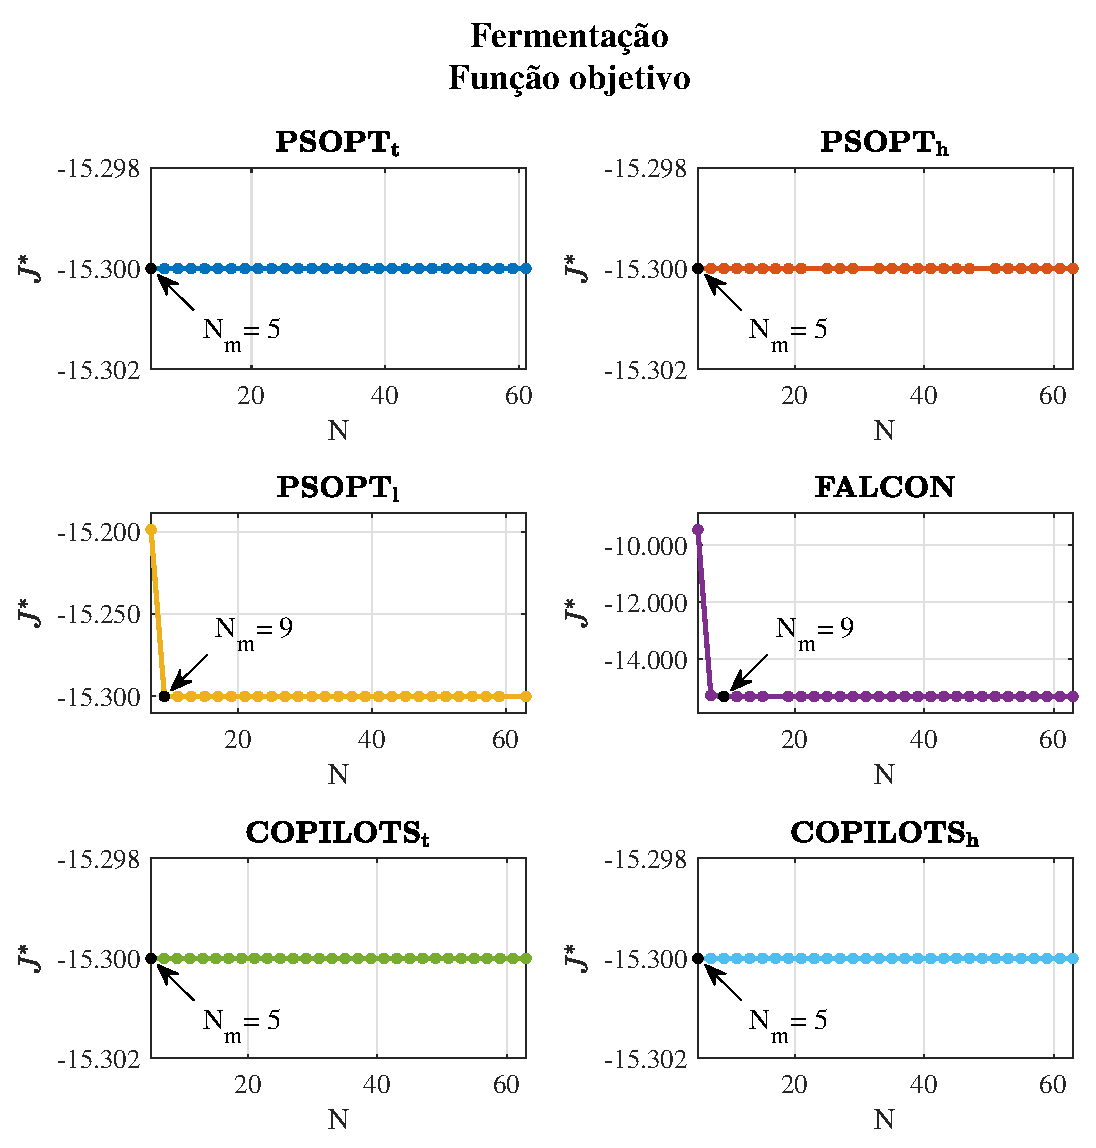
\includegraphics[scale=0.7]{fig/resultados/integrador/sens/J}
\captionof{figure}[Influência do número de nós de colocação no valor da função objetivo para o problema da aceleração de um bloco]{Influência do número de nós de colocação $N$ no valor da função objetivo $J^*$ para o problema da aceleração de um bloco.}
	\label{fig:integrador:sensibilidade:J}
	\vspace{\onelineskip}
\end{minipage}

Nestas figuras pode-se observar que, para o $ PSOPT_t $, $ FALCON $, e o $ COPILOTS_t $ (trapezoidal), o valor de $ J^* $ decresce à medida que $ N $ aumenta e se aproxima da solução analítica conhecida ($ J^* = 28 $). Já para o $ PSOPT_h $ e para o $ COPILOTS_h $ (Hermite-Simpson) e para o $ PSOPT_l $ (pseudo-espectral) observa-se que a solução é encontrada para $ N = 5 $. É importante ressaltar que, para a aplicação do método pseudo-espetral, não foi possível encontrar soluções para $ N $ iguais a 45, 47 e 53. Provavelmente, isto se deve a forma como foram inicializados os perfis das variáveis de estado e controle (\textcolor{red}{Arthur, por isso é importante destacar como essa inicialização é feita. A banca vai te questionar isso. Tem como mudar essa inicialização? Você tentou????. Uma pergunta, o processo de inicialização é o mesmo para todos????}).

Os resultados obtidos para esta aplicação são apresentados na Tabela \ref{tab:integrador:raw} para $ N = N_m$. Nesta tabela, $ t_p $ é o tempo de processamento médio, $ s_t $ é o desvio padrão atribuído a $ t_p $, $ n_{aval} $ é o número de avaliações da função objetivo, $ \Delta c_{max} $ é a máxima violação atribuída às restrições, $ N_s $ é o número de execuções bem sucedidas, e $ N_s\% $ é a relação entre $ N_s $ e o número total de execuções. 

\begin{table}
	\centering
	\caption[Métricas obtidas para o problema da aceleração de um bloco]{Métricas obtidas para o problema da aceleração de um bloco. Os melhores valores para $ N_m $, $ J^* $, $ t_p $, $ n_{aval} $ e $ N_s\% $ encontram-se destacados.}
	\label{tab:integrador:raw}
	\begin{tabular}{@{}ccccccccc@{}}
		\toprule
		Método       & $N_m$                             & $J^*$                                    & $t_p$ {[}$s${]}                         & $s_t$ {[}$s${]} & $n_{aval}$                        & $\Delta c_{max}$                         & $N_s$ & $N_s\%$                                  \\ \midrule
		$PSOPT_t$    & 35                                & 28,09170                                 & 0,31331                                 & 0,00625         & 8                                 & 6,41e-15                                 & 30    & {\color[HTML]{009901} \textbf{100,00\%}} \\
		$PSOPT_h$    & {\color[HTML]{009901} \textbf{5}} & {\color[HTML]{009901} \textbf{28,00000}} & 0,05395                                 & 0,00747         & 15                                & 4,44e-16                                 & 30    & {\color[HTML]{009901} \textbf{100,00\%}} \\
		$PSOPT_l$    & {\color[HTML]{009901} \textbf{5}} & {\color[HTML]{009901} \textbf{28,00000}} & 0,03791                                 & 0,00977         & {\color[HTML]{009901} \textbf{5}} & 7,77e-16                                 & 27    & 90,00\%                                  \\
		$FALCON$     & 35                                & 28,09167                                 & {\color[HTML]{009901} \textbf{0,03663}} & 0,00279         & 6                                 & 2,08e-16 & 30    & {\color[HTML]{009901} \textbf{100,00\%}} \\
		$COPILOTS_t$ & 35                                & 28,09167                                 & 0,52875                                 & 0,01817         & 1404                              & 1,57e-13                                 & 30    & {\color[HTML]{009901} \textbf{100,00\%}} \\
		$COPILOTS_h$ & {\color[HTML]{009901} \textbf{5}} & {\color[HTML]{009901} \textbf{28,00000}} & 0,18729                                 & 0,01770         & 600                               & 3,05e-13                                 & 30    & {\color[HTML]{009901} \textbf{100,00\%}} \\ \bottomrule
	\end{tabular}
\end{table}

Nesta tabela observa-se que foi necessário um maior valor para $ N $ para os pacotes que fazem uso da colocação trapezoidal ($ PSOPT_t $, $ FALCON $ e $ COPILOTS_t $) em comparação com os outros tipos de abordagens. Essa diferença se deve às características numéricas inerentes a cada método. Além disso, observa-se que os valores de $ J^* $ atribuídos às soluções obtidas por meio da colocação trapezoidal são bastante próximos uns dos outros.

Os maiores tempos de processamento foram atribuídos às soluções obtidas por meio do $ PSOPT_t $ e do $ COPILOTS_t $, uma vez que nesses casos foi utilizada uma quantidade maior de nós de colocação. Em contrapartida, o menor $ t_p $ foi encontrado pelo $ FALCON $. Esse comportamento se deve à capacidade que esse pacote possui de empregar ferramentas simbólicas na geração de derivadas analíticas, tanto para a função objetivo quanto para as restrições, o que leva a uma diminuição na quantidade de iterações despendida na obtenção da solução do problema em análise. A essa diminuição, está associada uma redução no tempo de processamento, mesmo quando utilizados muitos nós de colocação. Os tempos de processamento associados ao $ PSOPT_h $, $ PSOPT_l $, e $ FALCON $ foram bastante próximo e, consideravelmente, menores que aqueles requeridos pelo $ PSOPT_t $, $ COPILOTS_t $, e $ COPILOTS_h $. Vale ressaltar que, às soluções obtidas pelo $ COPILOTS $, normalmente estão associados a altos tempos de processamento, uma vez que o pacote utiliza o SQP e é escrito em Matlab\textsuperscript{\textregistered}.

Os valores de $ n_{aval} $ associados ao $ COPILOTS $, independentemente do tipo de colocação considerado, foram bem maiores que aqueles observados nos demais métodos avaliados, uma vez que o pacote faz uso do SQP. Observou-se também que nem sempre $ t_p $ está diretamente relacionado a $ n_{aval} $. Por exemplo, o tempo de processamento associado ao $ PSOPT_t $ é maior que aquele requerido pelo $ PSOPT_h $. Todavia, é o $ PSOPT_h $ que está associado com o maior $ n_{aval} $. Observa-se o mesmo comportamento quando são comparados os resultados obtidos pelo $ COPILOTS_t $ e pelo $ COPILOTS_h $. 

Por fim, ressalta-se que, utilizando qualquer um dos métodos, é possível obter soluções que satisfaçam as restrições do problema para quase todo $ N $. De fato, a $ N_s\% $ foram atribuídos valores iguais, ou bem próximos, a 100\%, enquanto $ \Delta c_{max} $ foi igual a  zero em todas estas execuções. Esse resultado se deve à simplicidade do problema, que não possui restrições terminais ou de caminho, o que na prática, implica em um problema mais simples. 

As trajetórias de estados considerando $ N = N_m $ são apresentadas nas Figuras \ref{fig:integrador:x:d} e \ref{fig:integrador:x:v}, e as trajetórias de controle na Figura \ref{fig:integrador:u:F}. A partir destes resultados constata-se que as trajetórias obtidas por cada um dos pacotes avaliados se mostraram similares. 

\noindent
\begin{minipage}{\textwidth}
	\vspace{\onelineskip}
	\centering
	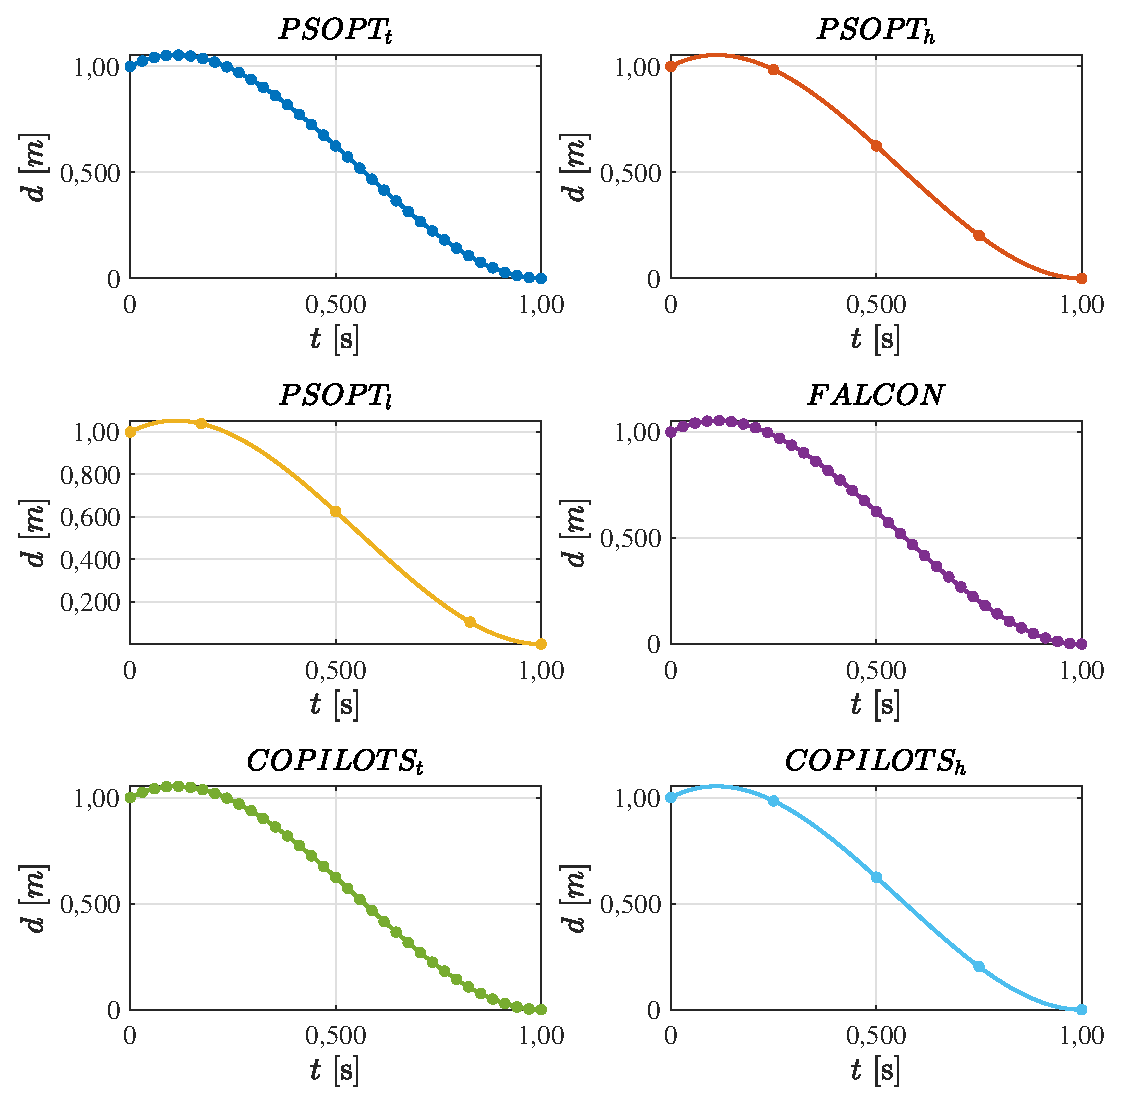
\includegraphics[scale=0.7]{fig/resultados/integrador/traj/x/d}
	\captionof{figure}[Variável de estado $d(t)$ para o problema da aceleração de um bloco]{Variável de estado $d(t)$ para o problema da aceleração de um bloco. Os pontos em cada um dos gráficos representam os valores discretizados, enquanto as linhas contínuas representam as trajetórias interpoladas.}
	\label{fig:integrador:x:d}
	\vspace{\onelineskip}
\end{minipage}

\noindent
\begin{minipage}{\textwidth}
	\vspace{\onelineskip}
	\centering
	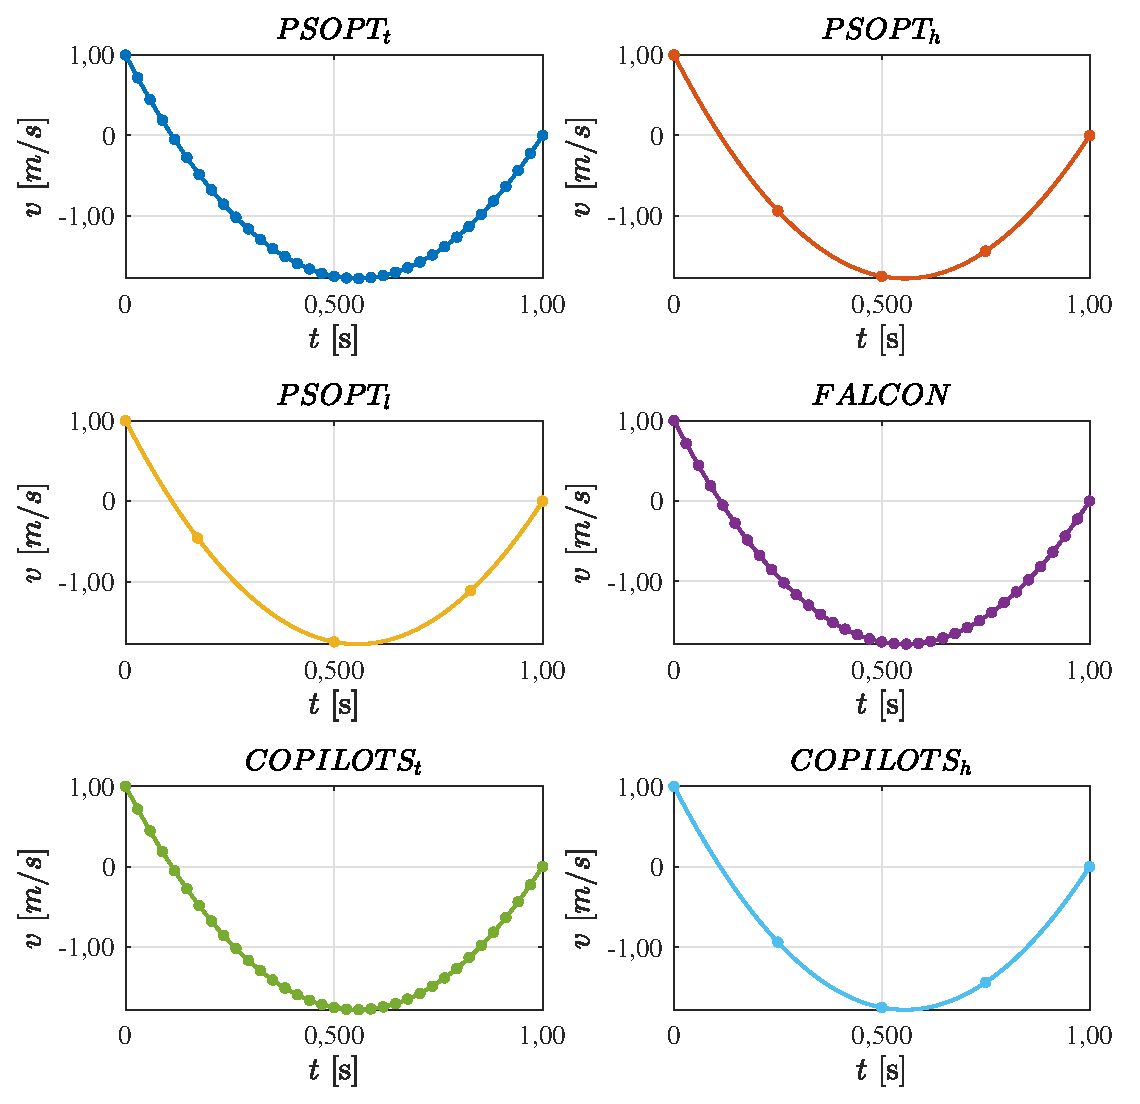
\includegraphics[scale=0.7]{fig/resultados/integrador/traj/x/v}
	\captionof{figure}[Variável de estado $v(t)$ para o problema da aceleração de um bloco]{Variável de estado $v(t)$ para o problema da aceleração de um bloco. Os pontos em cada um dos gráficos representam os valores discretizados, enquanto as linhas contínuas representam as trajetórias interpoladas.}
	\label{fig:integrador:x:v}
	\vspace{\onelineskip}
\end{minipage}

A influência do aumento do número de nós de colocação no tempo de processamento e no número de avaliações da função objetivo são apresentadas nas Figuras \ref{fig:integrador:sensibilidade:t} e \ref{fig:integrador:sensibilidade:naval}, respectivamente. Acima de cada um dos gráficos são apresentadas as diferenças entre os valores máximo e mínimo associados à métrica em questão ($ t_p $ ou $ n_{aval} $), isto é: $ \Delta t_p = \max\{t_p\} - \min\{t_p\} $ e $ \Delta n_{aval} = \max\{n_{aval}\} - \min\{n_{aval}\} $. Os pontos nos gráficos representam os valores obtidos para $ t_p $ (e $ n_{aval} $) em cada nó de colocação, enquanto as linhas contínuas representam curvas de tendência, obtidas por meio de regressões lineares, sendo a sua concordância avaliada de acordo com o coeficiente de determinação ($R^2$). Os valores de $ N $ empregados na geração desses dados são iguais àqueles considerados na computação da relação entre $ J^* $ e $ N $. 

\noindent
\begin{minipage}{\textwidth}
	\vspace{\onelineskip}
	\centering
	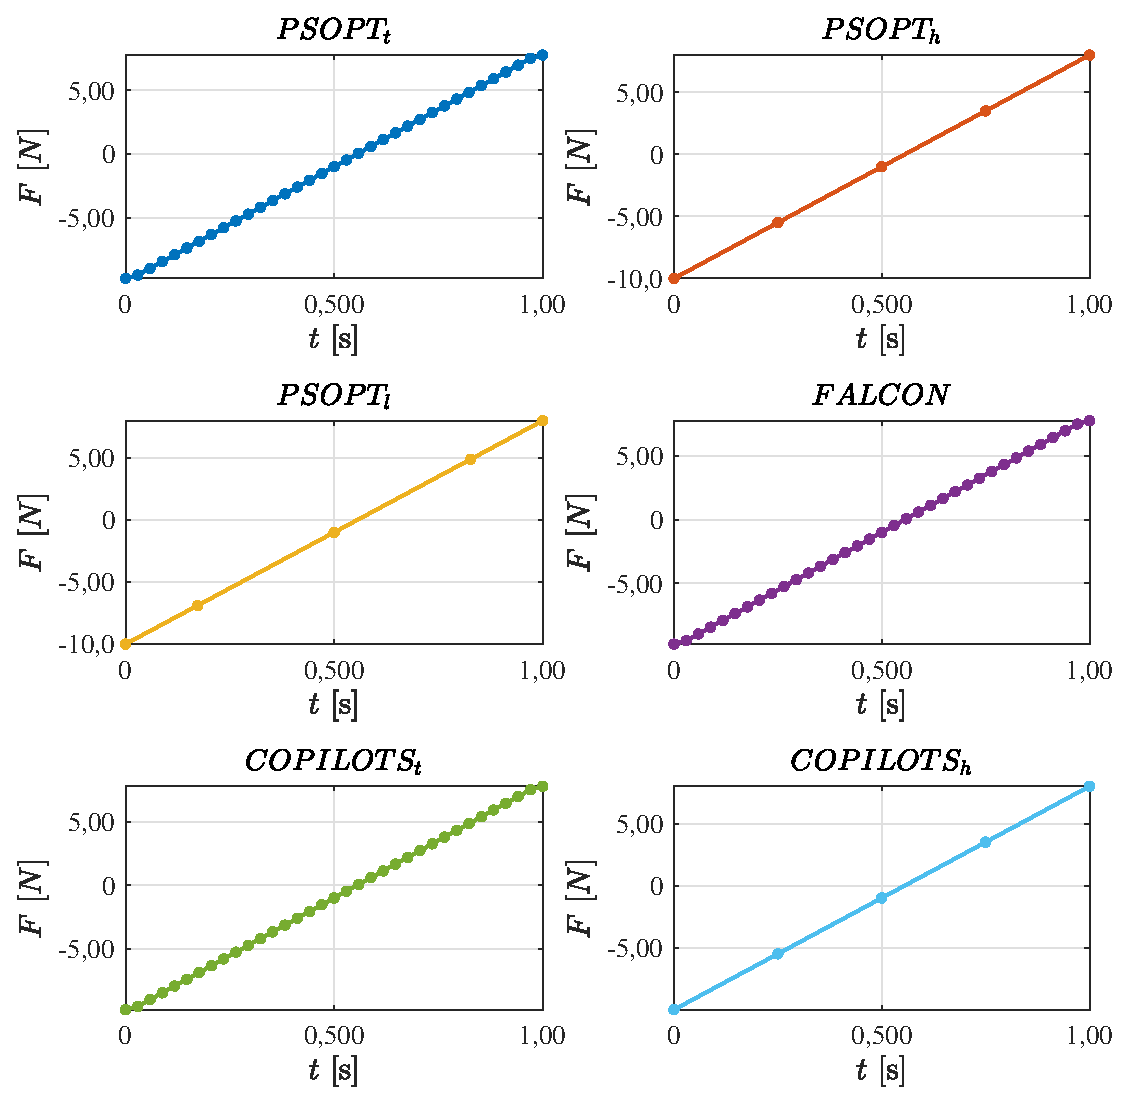
\includegraphics[scale=0.7]{fig/resultados/integrador/traj/u/F}
	\captionof{figure}[Variável de controle $F(t)$ para o problema da aceleração de um bloco]{Variável de controle $F(t)$ para o problema da aceleração de um bloco. Os pontos em cada um dos gráficos representam os valores discretizados, enquanto as linhas contínuas representam as trajetórias interpoladas.}
	\label{fig:integrador:u:F}
	\vspace{\onelineskip}
\end{minipage}

De forma geral nesta figura observa-se o aumento do número de nós de colocação implicam, como esperado, no aumento do tempo de processamento. Em relação ao $ PSOPT_t $ e ao $ PSOPT_h $, estes apresentam tempos de processamento similares e bem inferiores em relação ao $ PSOPT_l$. Já para o $ COPILOTS_t$ observam-se, em média, tempos de processamentos bem distintos em relação ao $ COPILOTS_h$ e aos outros pacotes. Este maior tempo de processamento esta relacionado à solução do PPNL resultante da etapa de discretização. Já para o $ FALCON $ observa-se que este pacote se mostrou muito pouco sensíveis ao aumento de $ N $. Tal fato pode ser justificado ao uso de ferramentas simbólicas na obtenção de derivadas analíticas. De forma geral, apesar das diferenças entre os tempos de processamentos médios observados, considera-se que ambos os pacotes foram eficientes na resolução do problema em questão, visto que a magnitude dos tempos médios requeridos são condizentes com os esperados.

\noindent
\begin{minipage}{\textwidth}
	\vspace{\onelineskip}
	\centering
	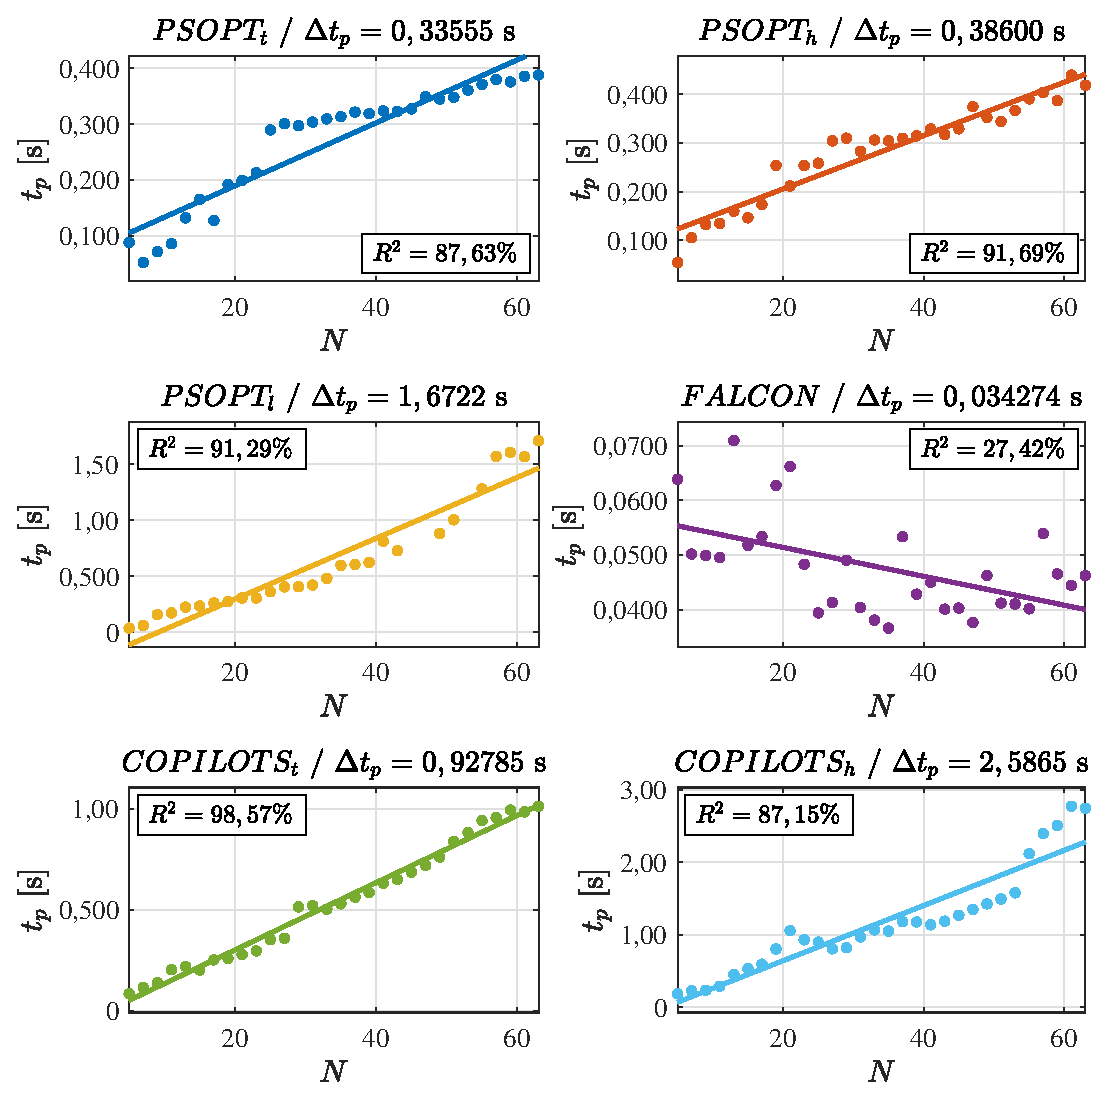
\includegraphics[scale=0.7]{fig/resultados/integrador/sens/t}
	\captionof{figure}[Relação entre o tempo de processamento e o número de nós de colocação para o problema da aceleração de um bloco]{Relação entre o tempo de processamento $ t_p $ e o número de nós de colocação $ N $ para o problema da aceleração de um bloco.}
	\label{fig:integrador:sensibilidade:t}
	\vspace{\onelineskip}
\end{minipage}

Com relação ao número de avaliações da função objetivo ($ n_{aval} $), a variação observada para este parâmetro foi praticamente a mesma para o $ PSOPT_t$, $ PSOPT_h$ e $FALCON$. Já observa-se um aumento significativo para o $ PSOPT_l$ em relação a estes. Os maiores valores para estas variações são observadas para as duas configurações do $COPILOTS$. Este incremento no valor deste parâmetro está associado à solução do PPNL, conforme destacado anteriormente para a análise do  tempo de processamento. Naturalmente, com o aumento no número de nós tem-se o aumento do parâmetro $n_{aval}$, conforme pode ser observado para o $ PSOPT_l$, $COPILOTS_t$ e $COPILOTS_h$. Todavia, para os pacotes $ PSOPT_t$, $ PSOPT_h$ e o $FALCON$, é possível observar uma pequena flutuação no valor de $ n_{aval} $ quando $N$ aumenta. Isto não quer dizer que, para estas variantes, o aumento na discretização do método numérico implique na redução do número de avaliações requeridas, mas apenas que existe uma flutuação neste valor que é função das condições iniciais associadas, bem como na estratégia implementada em cada para a resolução do PCO.

\noindent
\begin{minipage}{\textwidth}
	\vspace{\onelineskip}
	\centering
	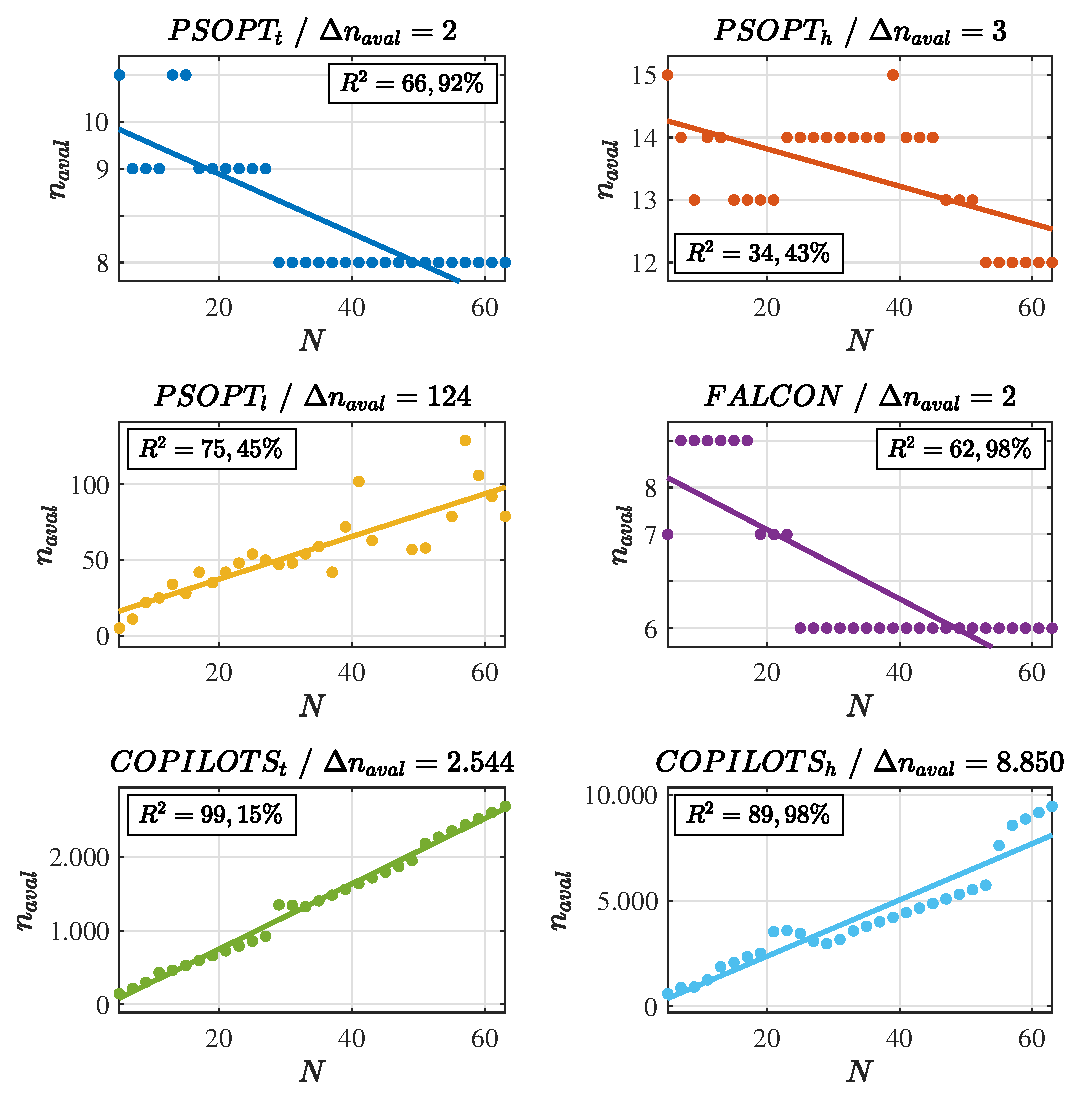
\includegraphics[scale=0.7]{fig/resultados/integrador/sens/eval}
	\captionof{figure}[Relação entre o número de avaliações da função objetivo e o número de nós de colocação para o problema da aceleração de um bloco]{Relação entre o número de avaliações da função objetivo $ n_{aval} $ e o número de nós de colocação $ N $ para o problema da aceleração de um bloco.}
	\label{fig:integrador:sensibilidade:naval}
	\vspace{\onelineskip}
\end{minipage}